\documentclass[10pt,twocolumn,letterpaper]{article}

\usepackage{iccv}
\usepackage{times}
\usepackage{epsfig}
\usepackage{graphicx}
\usepackage{amsmath}
\usepackage{amssymb}
\usepackage{bbm}
\usepackage{ccmap}
% Include other packages here, before hyperref.

\usepackage{color}
\usepackage{enumerate}


\newcommand{\cxj}[1]{\textcolor[rgb]{1.00,0.00,0.00}{(cxj: #1)}}
\newcommand{\mdf}[1]{\textcolor[rgb]{0.00,0.00,1.00}{#1}}
\newcommand{\bobo}[1]{\textcolor[rgb]{0.00,0.30,0.00}{(mbobo: #1)}}
\newcommand{\que}[1]{\textcolor[rgb]{0.00,0.30,0.00}{#1}}
\newcommand{\vb}[1]{\mathbf{#1}}
\newcommand{\comments}[1]{}


% If you comment hyperref and then uncomment it, you should delete
% egpaper.aux before re-running latex.  (Or just hit 'q' on the first latex
% run, let it finish, and you should be clear).
\usepackage[pagebackref=true,breaklinks=true,letterpaper=true,colorlinks,bookmarks=false]{hyperref}

% \iccvfinalcopy % *** Uncomment this line for the final submission

\def\iccvPaperID{****} % *** Enter the ICCV Paper ID here
\def\httilde{\mbox{\tt\raisebox{-.5ex}{\symbol{126}}}}

% Pages are numbered in submission mode, and unnumbered in camera-ready
\ificcvfinal\pagestyle{empty}\fi
\begin{document}

%%%%%%%%% TITLE
\title{Deep Shape-Aware Network for Objects Segmentation with Prior Shape Knowledge}

\author{First Author\\
Institution1\\
Institution1 address\\
{\tt\small firstauthor@i1.org}
% For a paper whose authors are all at the same institution,
% omit the following lines up until the closing ``}''.
% Additional authors and addresses can be added with ``\and'',
% just like the second author.
% To save space, use either the email address or home page, not both
\and
Second Author\\
Institution2\\d
First line of institution2 address\\
{\tt\small secondauthor@i2.org}
}

\maketitle
%\thispagestyle{empty}


%%%%%%%%% ABSTRACT
\begin{abstract}
   Accurate segmentation of biomembrane objects is a crucial step to obtain morphological statistics in biomedical analysis.
   However in many scenarios, prior shape knowledge about biomedical objects is available, which is useful for resolving the coarse boundary and touching problem.
   In this paper, we introduce a novel Deep Shape-Aware Network (DSAN) by absorbing prior shape knowledge about plausible components into the network.
   Our SCNN is a multi-task framework that simultaneously predicts an objectness score and several shape parameters as auxiliary at each pixel.
   The auxiliary predictions formulate the shape of each object, which can not only separate segmented objects into individual ones, but also optimize their boundary in terms of prior shape knowledge.
   Furthermore, a novel split pooling operation is developed to optimize both objectness scores and shape parameters to produce a better segmentation masks.
   The whole process is efficient and trained end-to-end.
   Experiments on two challenging biomedical problems, including synaptic vesicles and histopathological glands segmentation, demonstrate the effectiveness of our approach.
   And we expect our method to empower more works to incorporate various prior knowledge into neural networks to benefit their researches.

\end{abstract}

%%%%%%%%% BODY TEXT
\section{Introduction}
Recent advances in biomedical image analysis have assisted many pathologists and biologists to facilitate their researches \cite{Chen2016b, Ronneberger2015,Chen2016c,Lieman-Sifry2017,Paszke2016,Tseng2017,Sirinukunwattana2015b}.
Among these researches, a significant application is to obtain the accurate segmentation of specific membrane objects in a biomedical image, such as lumenal glands, synaptic vesicles and cells.
Especially, the morphological shape and spatial distribution of synaptic vesicles are helpful to study the neural activity in different brain regions, while morphological statistics of lumenal glands are widely used for assessment of the malignancy degree of adenocarcinomas.
%
Conventionally, these crucial steps are performed by human expert, which are time-consuming and suffer from subjective factors.
\cxj{For example, how long does it take to handle a task..?}
Therefore, it is significantly demanded to improve the efficiency as well as the reliability with automatic segmentation methods.

\begin{figure}
    \begin{center}
        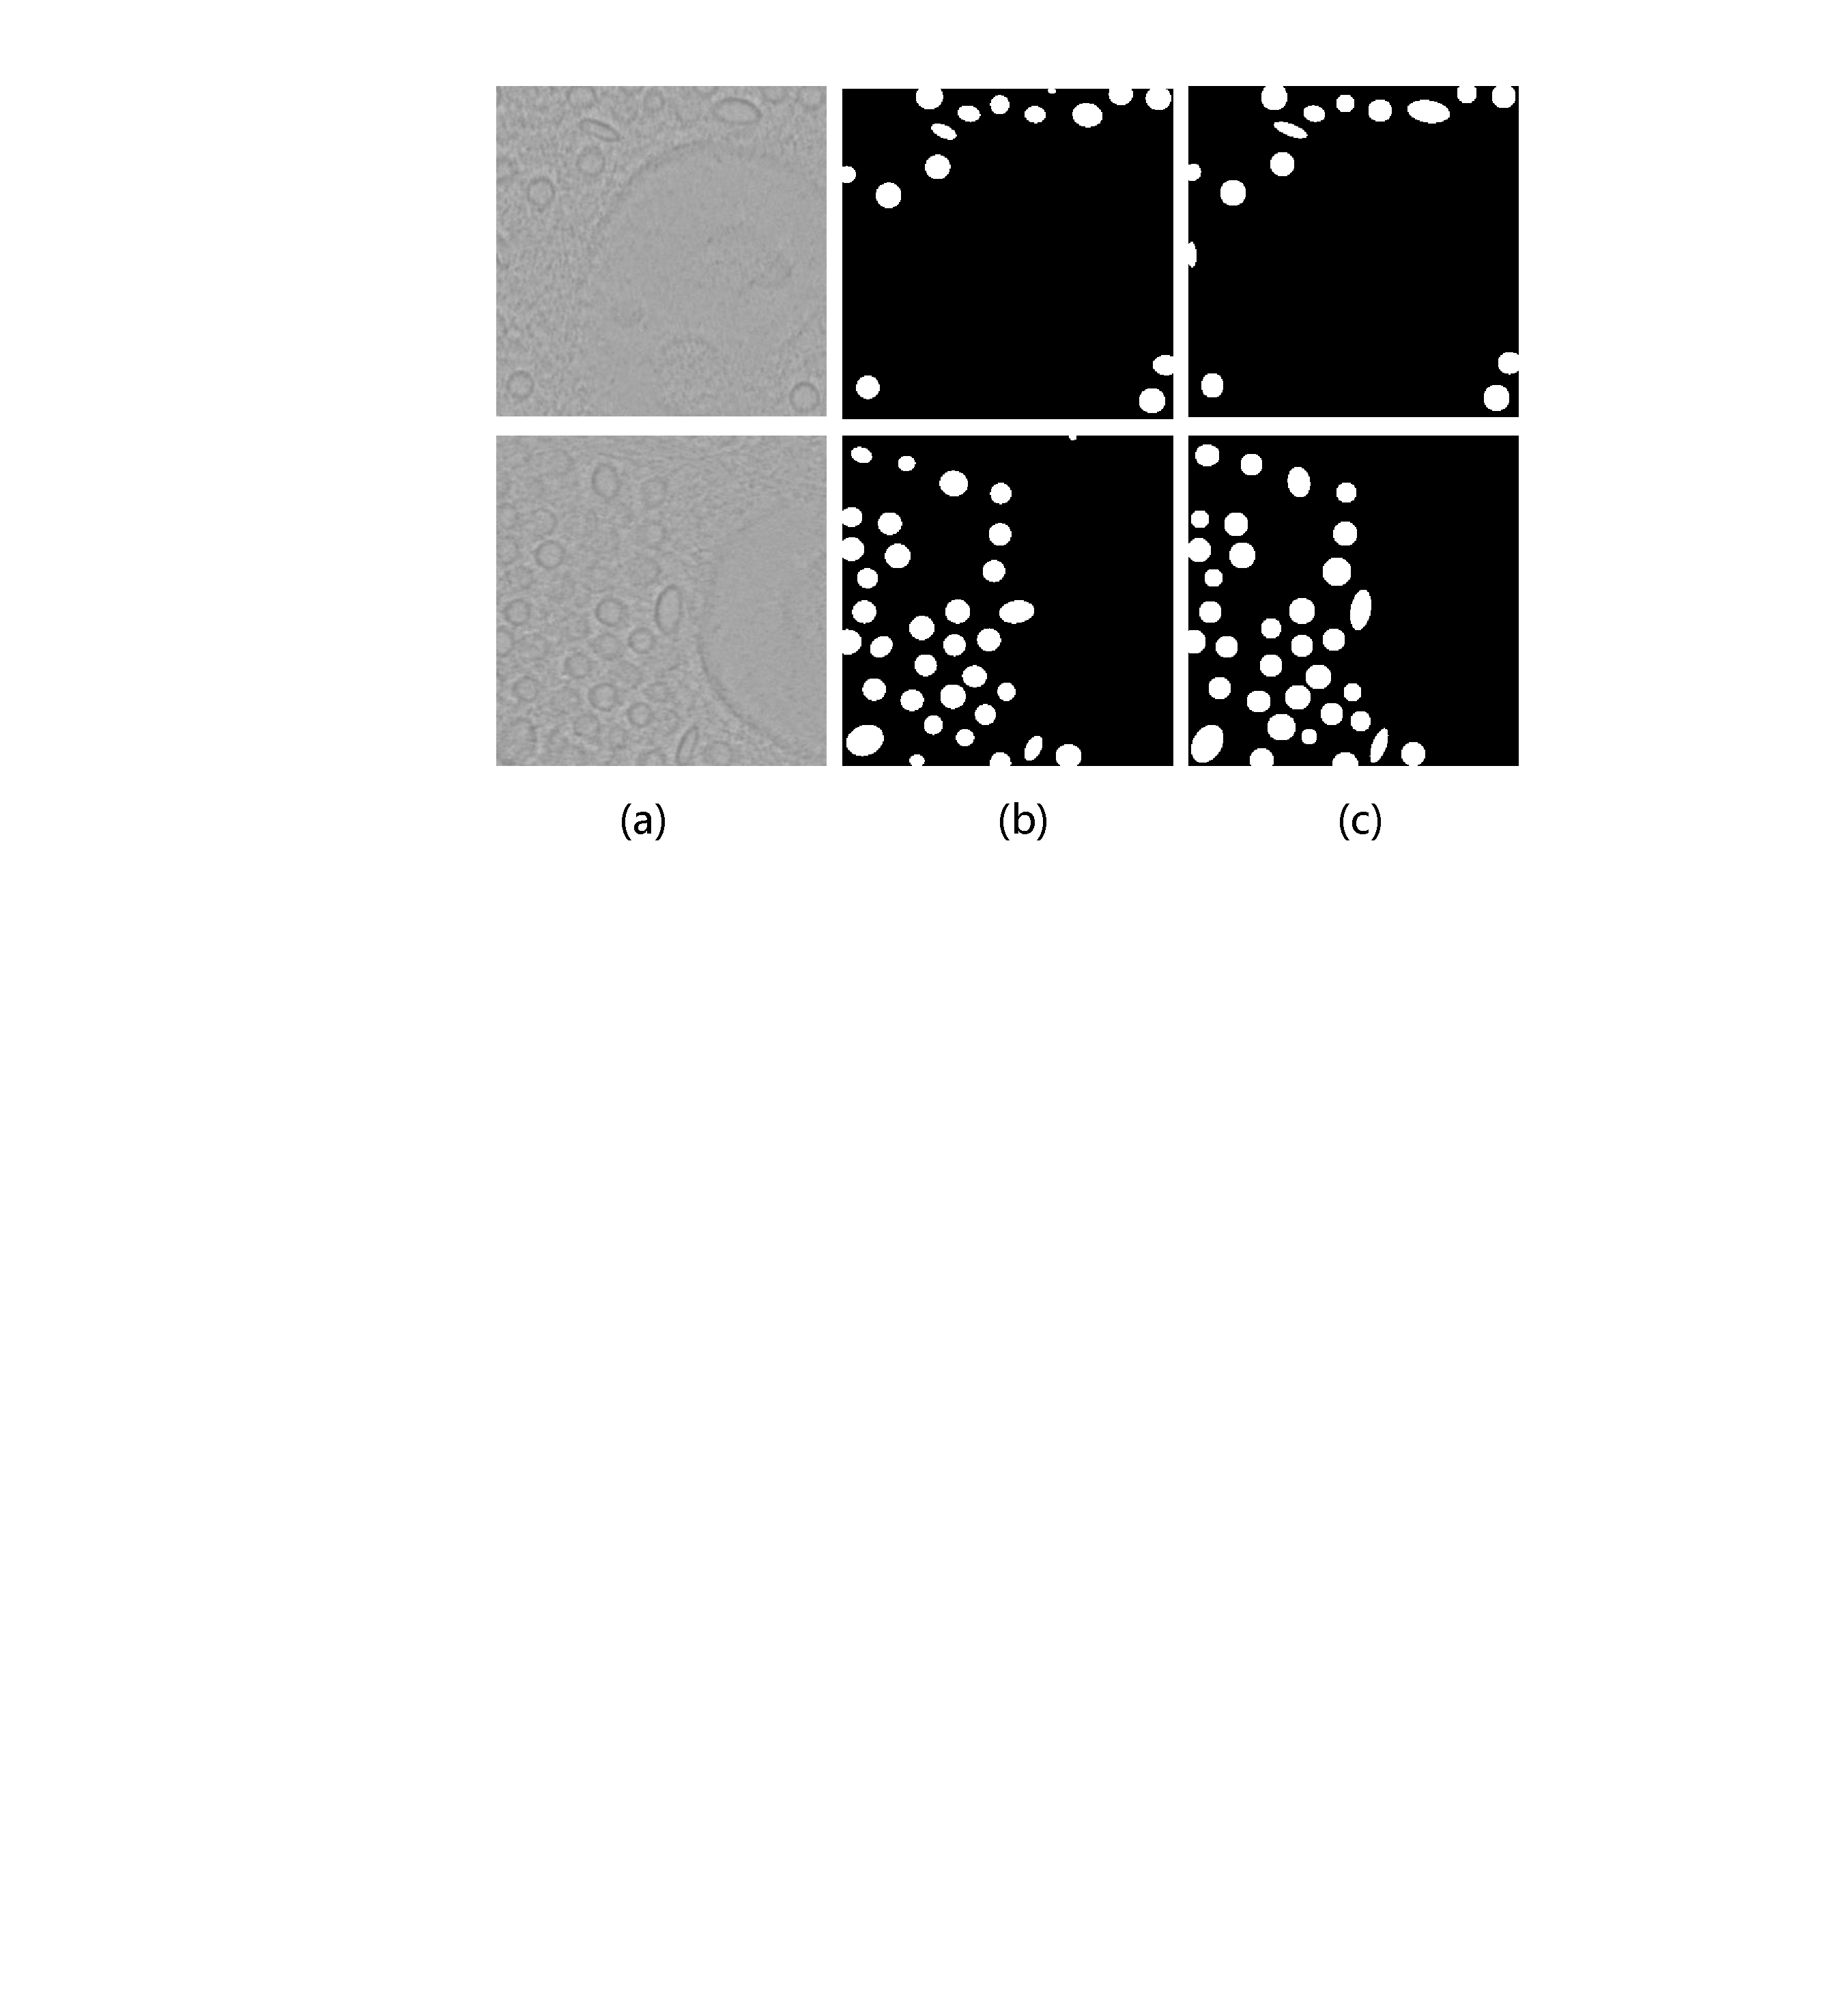
\includegraphics[width=3.3in]{figures/FigImg.pdf}
    \end{center}
    \caption{An example showing the challenges of biomedical segmentation: (a) synaptic vesicle image; (b) results from proposed SCNN by incorporating prior shape knowledge; (c) annotations by experts.}
    \label{FigImgs}
\end{figure}

However, it is non-trivial to automatically segment biomedical images.
First, biomedical images are usually noisy and obscure caused by deficient imaging techniques, as shown in Figure~\ref{FigImgs} (a).
Second, most membrane objects in biomedical images are arranged compactly and densely arrangement, thus it is hard to separate objects individually, which is known as the touching problem.
Third, in some pathological cases, the inter-class deformation of some pathological objects are much different, while the shape of most healthy objects are regular.
It is hard to incorporate prior shape knowledge to optimize most regular objects without restricting the model generalization to pathological cases \cite{Sirinukunwattana2015b}.

Recently, deep neural networks have demonstrated excellent performance in biomedical image segmentation with the use of fully convolutional networks \cite{Dhungel2015,Ronneberger2015,Roth2015,Chen2015,Lieman-Sifry2017,Xu2016,Chen2016b}.
However, as most of these deep networks are based on fully convolutional networks~\cite{Long2015}, the pooling and downsampling layers make them inevitable to get poorly localized object boundaries.
To increase the boundary accuracy, many efforts have been made recently. An U-shaped deep network called U-net~\cite{Ronneberger2015} is proposed for biomedical image segmentation. 
By employing the skip connections between contracting and expanding paths, context information can be directly propagated to higher resolution layers for detail preserving.
Several improvements of U-net were proposed soon afterwards.
DeepVentricle~\cite{Lieman-Sifry2017}, which uses the same padding instead of valid padding, has been successfully used for cardiac segmentation.
Recently, DCAN~\cite{Chen2016a} integrates complementary information of objects and contours in a multi-task learning framework to separate the clustered objects into individual ones.\cxj{for more accurate boundaries?}
Although these methods achieved promising results in their segmentation tasks, they may fail to achieving satisfying performance in denser and smaller objects with regular shapes, such as synaptic vesicle dataset shown in Figure~\ref{FigImgs}.

In this paper, we propose a first Shape-Constrained neural network (SCNN) to segment dense objects by inherently incorporating prior shape knowledge into network.
Similar with \cite{Chen2016a}, we formulate the network as a multi-task learning framework by simultaneously predicting an objectness scores map and an auxiliary map for an input image.
Instead of contour probability \cite{Chen2016a,Chen2016,Bertasius2016}, our SCNN learns the parameterized expression of objects shape, which emphasizes more on the overall shape of objects.
Inspired by Region Proposal Networks in \cite{Ren2015}, our SCNN simultaneously predicts objectness scores and a set of shape parameters, which formulate the shape of a nearest object, at each position.
The complementary information in auxiliary parameters can not only separate objects into individual ones, but also optimize their shapes.

However since the objects are not always regular, their shape cannot be parameterized uniformly and constrained strictly.
Therefore, we select a best representative shape as constraint and adopt a local optimizing strategy in fusion step to find a balance between regularization and unconstraint.
In this way, our SCNN not only optimizes the segmentation of regular objects with prior shape knowledge, but also well accommodates serious deformable objects.
\cxj{what do you mean here?}

Furthermore, predicting the shape parameters of objects accurately is a significantly challenge task, because complex information is required to analyze the overall context of a neighbouring object
\cxj{Why this is more difficult? what is the challenge?}
To this end, we proposed a novel joint max pooling to improve the performance of both objectness scores and shape parameters in final fusion step by exploring the intrinsic correlation between them.
Moverover, JMP is designed as a trainable layer, which can be trained end-to-end and easily extended to any multi-task networks.

\begin{figure}
    \begin{center}
        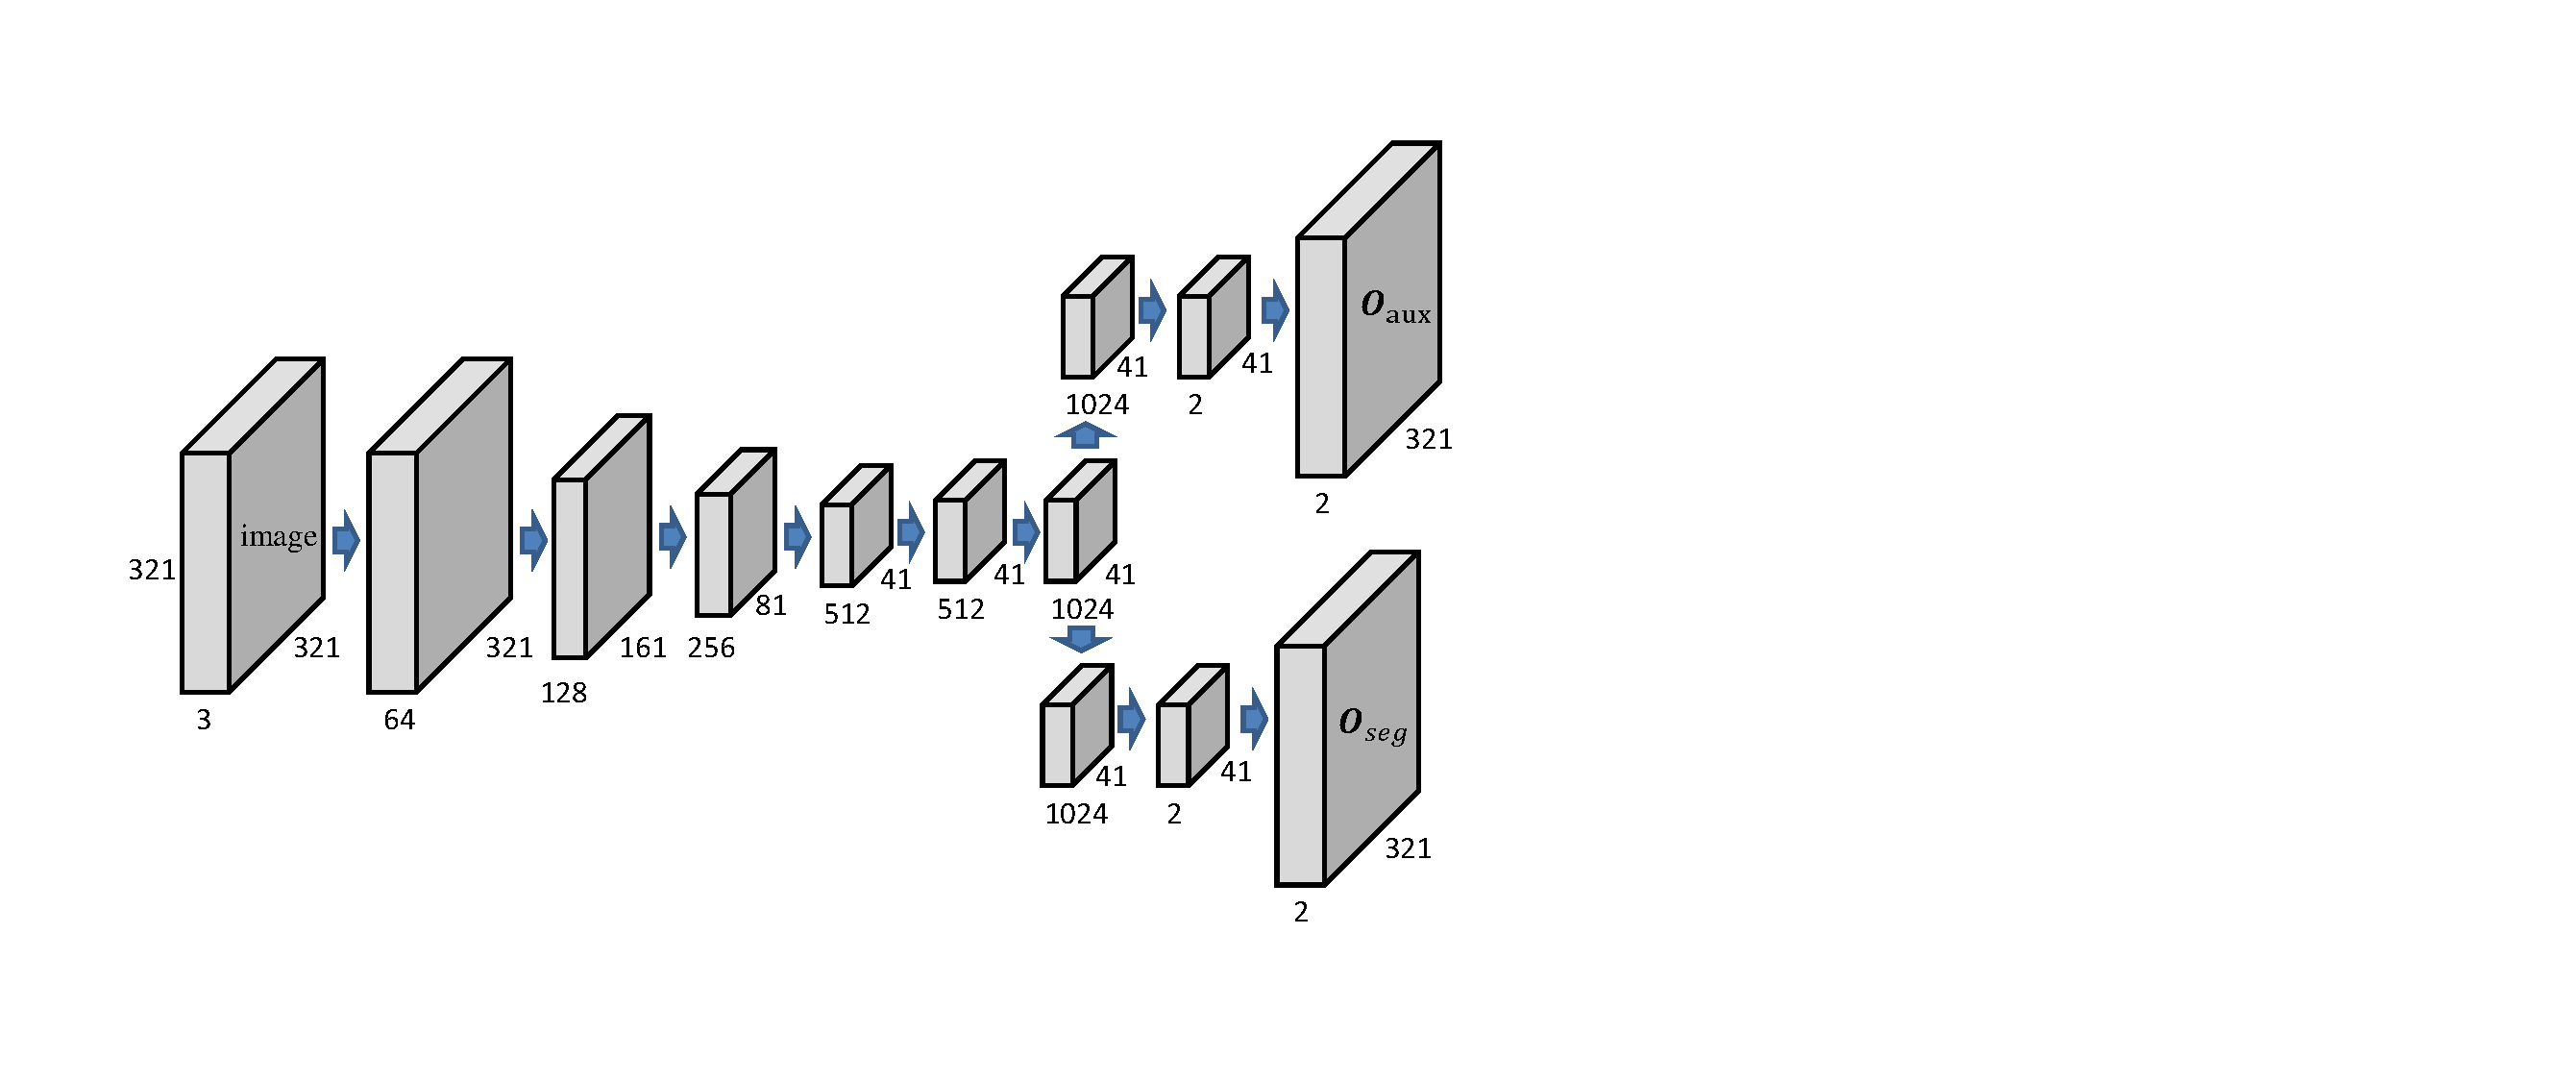
\includegraphics[width=3.3in]{figures/FigMTN.pdf}
    \end{center}
    \caption{Architecture of multi-task neural network based on FCN. \cxj{I would sugest using real images as input and output.}}
    \label{FigMTN}
\end{figure}
Overall, the contribution of this paper is three-fold:
\begin{enumerate}
	\item We first effectively incorporate shape constraint into deep neural networks.
	% for biomedical image segmentation.
	\item We propose a novel joint max pooling for benefiting both multi-task outputs.
	\item Our framework is applicable to a series of different tasks such as biomedical image segmentation, scent detection task and achieves the state-of-the-art performance.
\end{enumerate}
\section{Proposed Method}
\label{sec:method}

A complete pipeline of Shape-Constrained Neural Network (SCNN) is illustrated in Figure~\ref{FigSCNN}.
The framework is trained end-to-end and consists of three key components:
1) a multi-task neural network based on FCN,
2) proposed joint max pooling and
3) local optimizing strategy to fuse the multi-outputs into final segmentation mask.
%
\begin{figure*}
    \begin{center}
        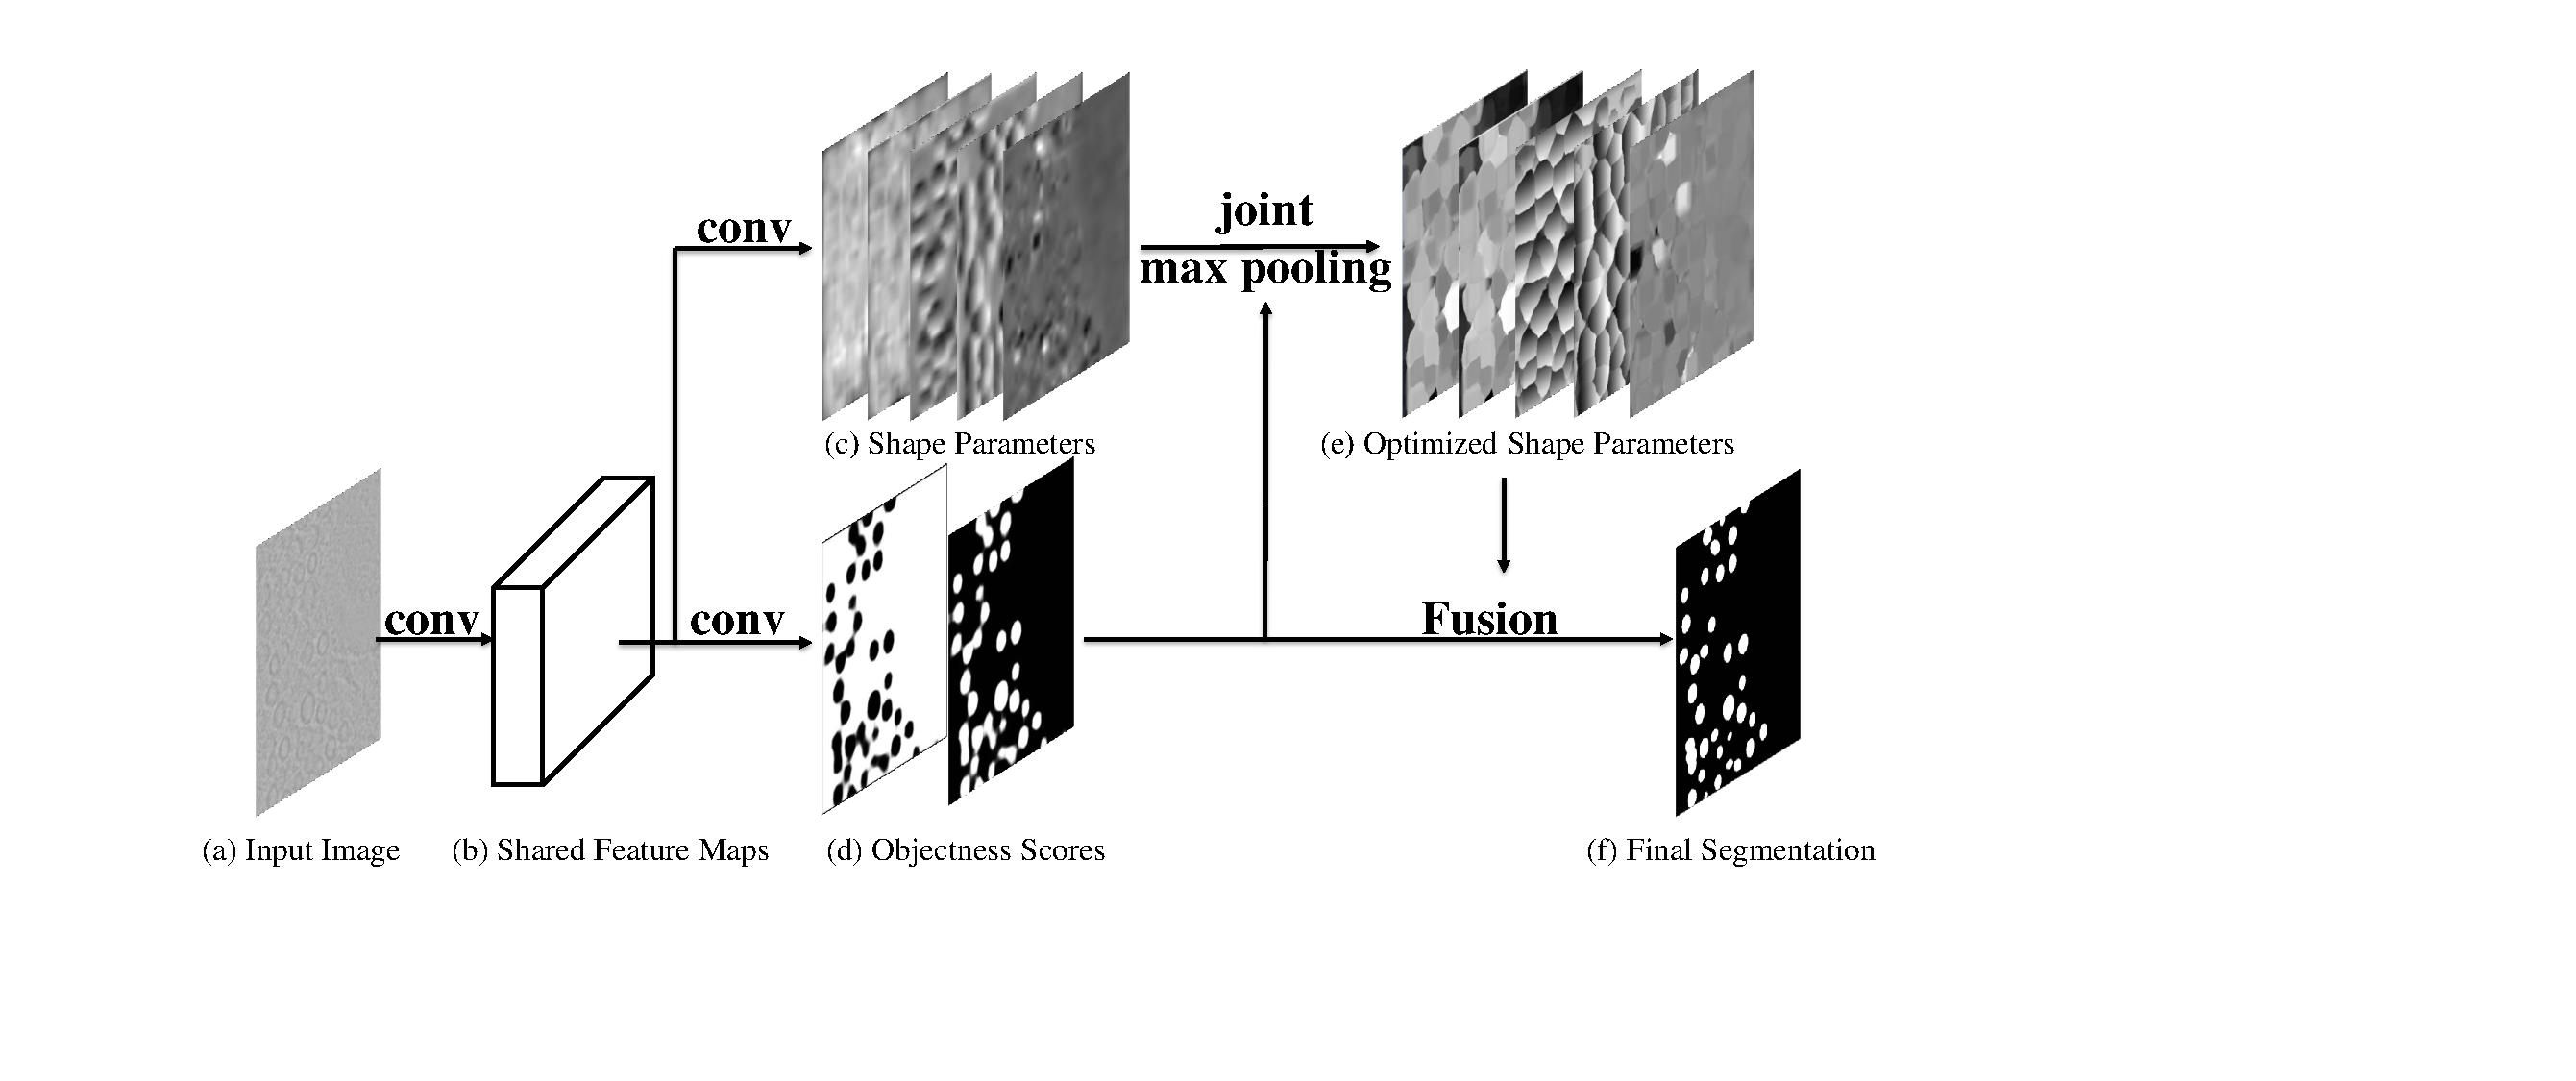
\includegraphics[width=6.8in]{figures/FigSCNN.pdf}
    \end{center}
    \caption{Overview of our proposed scnet. Given an image (a), multi-task neural network simultaneously predict objectness scores (d) and shape parameters of objects (d) using shared feature maps (b).
    Then a joint max pooling is applied to pool (c) with (d) and output new shape parameters (e).
    Finally, segmentation mask (f) is obtained by fusing objectness (d) with the parameterized contour description (e).}
    \label{FigSCNN}
\end{figure*}

Given an input image, the first part is a multi-task FCN which separately predicts objectness scores and shape parameters maps (Sec.~\ref{sec:multi-task-fcn}).
Then two branches integrate with each other by a joint max pooling layer (Sec.~\ref{sec:joint-max-pooling}) and a local fusion step to finally predict the shape-constrained segmentation (Sec.~\ref{sec:fusion}).

\subsection{Multi-task FCN}
\label{sec:multi-task-fcn}

The architecture of our multi-task learning network is shown in Figure~\ref{FigMTN}.
It simultaneously predicts an objectness map $p$ and an auxiliary map $t$ as complementary information.
The feature extracting part is shared and based on the publicly available DeepLab model~\cite{Chen2014a}, which introduces zeros into the filters to enlarge its Field-of-View.
Subsequently, extracted feature maps of last shared convolution layer are fed into two individual branches.
In each branch, successive two convolution layers, respectively with kernel size of $3\times3$ and $1\times1$, are applied to shared feature map, and then an upsampling layer restores their resolution to the input image size.
During training, the parameters of shared layers are jointly optimized, while the parameters of two branches are updated separately.

Instead of directly predicting contour probabilities like \cite{Chen2016a,Xu2016}, we choose the parameterized expression of objects shape as our complementary information, which emphasizes more on the overall shape of an object.
For example in our task for vesicle segmentation, the ellipse shape is applied as our prior shape knowledge and formulated by $5$ parameters: $\{\theta, \mu_c, \nu_c, a, b\}$.
$\theta$ is the rotated angle of the major axis from $x-$axis.
$(\mu_c, \nu_c)$ are the coordinates of elliptical center.
And $a$, $b$ are respectively the lengths of the major and minor axis.
With this definition, our auxiliary map $p$ has $5$ channels, each of which corresponds to one parameter.
For better regression, we further normalize the shape parameters by image width and height so that they fall in $[0,1]$:
\begin{eqnarray}\label{EqMax}
\begin{aligned}
p_i= \{\theta,\frac{\mu-\mu_c}{w},\frac{\nu-\nu_c}{h},\frac{a}{w},\frac{b}{h}\}
\end{aligned}
\end{eqnarray}
where $p_i$ is a vector regressed on position $i$, consisting of shape parameters of a nearest object.
$(\mu, \nu)$ are spatial coordinates of $p_i$.
and $w$,$h$ are image width and height.

The objective function follows the multi-task loss in~\cite{Ren2015}.
Our loss of multi-task FCN for an image is defined by:
\begin{eqnarray}\label{EqLoss}
\begin{aligned}
L(p,t) &= \frac{1}{N}(\sum_{i}L_{cls}(p_i,p^*_{i})+\lambda\sum_{i}p^*_{i}L_{reg}(t_{i},t^*_{i}))
\end{aligned}
\end{eqnarray}
where $N$ is the pixel number of input image.
$p^*_i$ and $t^*_i$ are the ground truth of objectness score and shape parameters.
The classification loss $L_{cls}$ is a soft-max loss over different classes.
And the regression loss $L_{reg}$ is the smooth $L_1$ loss in \cite{Ren2015} defined by
\begin{eqnarray}
\label{EqSmoothL1}
\begin{aligned}
L_{reg}(t_i,t^*_{i}) =\left\{\begin{array}{cc}
|t_i-t^*_{i}|&if~|t_{i}-t^*_{i}|>1\\
\frac{1}{2}(t_{i}-t^*_{i})^2&else\\
\end{array}\right.
\end{aligned}
\end{eqnarray}

Especially, we only consider the regression loss with positive $p^*_i$ in Eq.~\ref{EqLoss}, because most predicted $t_i$ with negative $p^*_i$ will be abandoned in next section by proposed joint max pooling.
And $\lambda$ is a balancing weight between $L_{cls}$ and $L_{reg}$.

\subsection{Joint Max Pooling}
\label{sec:joint-max-pooling}

Obtained from two individual branches of multi-task FCN, objectness and auxiliary map of shape parameters are coarse and uncorrelated \bobo{Is it not strict by using 'uncorrelated' because there should be a bond by shared feature extracting}.
Especially in auxiliary map, only predicted shape parameters in central area of objects satisfy the requirement of accuracy.
This is caused by intrinsic challenge for exploring the objects shape and different perception field needed by different position to predict the integral shape of the nearest object.
To this end, we introduce a novel joint max pooling (JMP) to improve the accuracy of auxiliary predictions in border area of the objects, where is useful to next fusion step.
Different from conventional max pooling, our JMP takes both auxiliary and objectness maps as inputs and pools the former map with the latter, of which the back propagation further benefits to both inputs by exploring their inherent association.
\cxj{not clear about your key idea. You need one sentence to describe your main idea of joint pooling, how does it combine two maps.}

A conventional pooling operation can expressed as
\begin{eqnarray}\label{pooling}
\begin{aligned}
y_{j} = \sum_{i\in \mathcal{N}_{j}} \omega_{i}x_{i}
\end{aligned}
\end{eqnarray}
where $\mathcal{N}_{j}$ is a neighbor region of pixel $j$ according to the sliding window, and $\omega_{i}$ is the weight of pixel $i$.
For traditional max pooling, $\omega_i \in \{0,1\}$ is a binary indicator for that if $x_i$ is the maximum in the local region.
There is only one pixel in the neighborhood has $\omega=1$ and all the others have $\omega=0$.
For an average pooling, all pixels in the local window take the identical weight $\omega=\frac{1}{N}$, where $N$ is the total number of pixels in the local region $\mathcal{N}$.
Intuitively, $\omega$ acts like an "indictor" determining which $x$ should be propagated to next layer.

\begin{figure}
    \begin{center}
        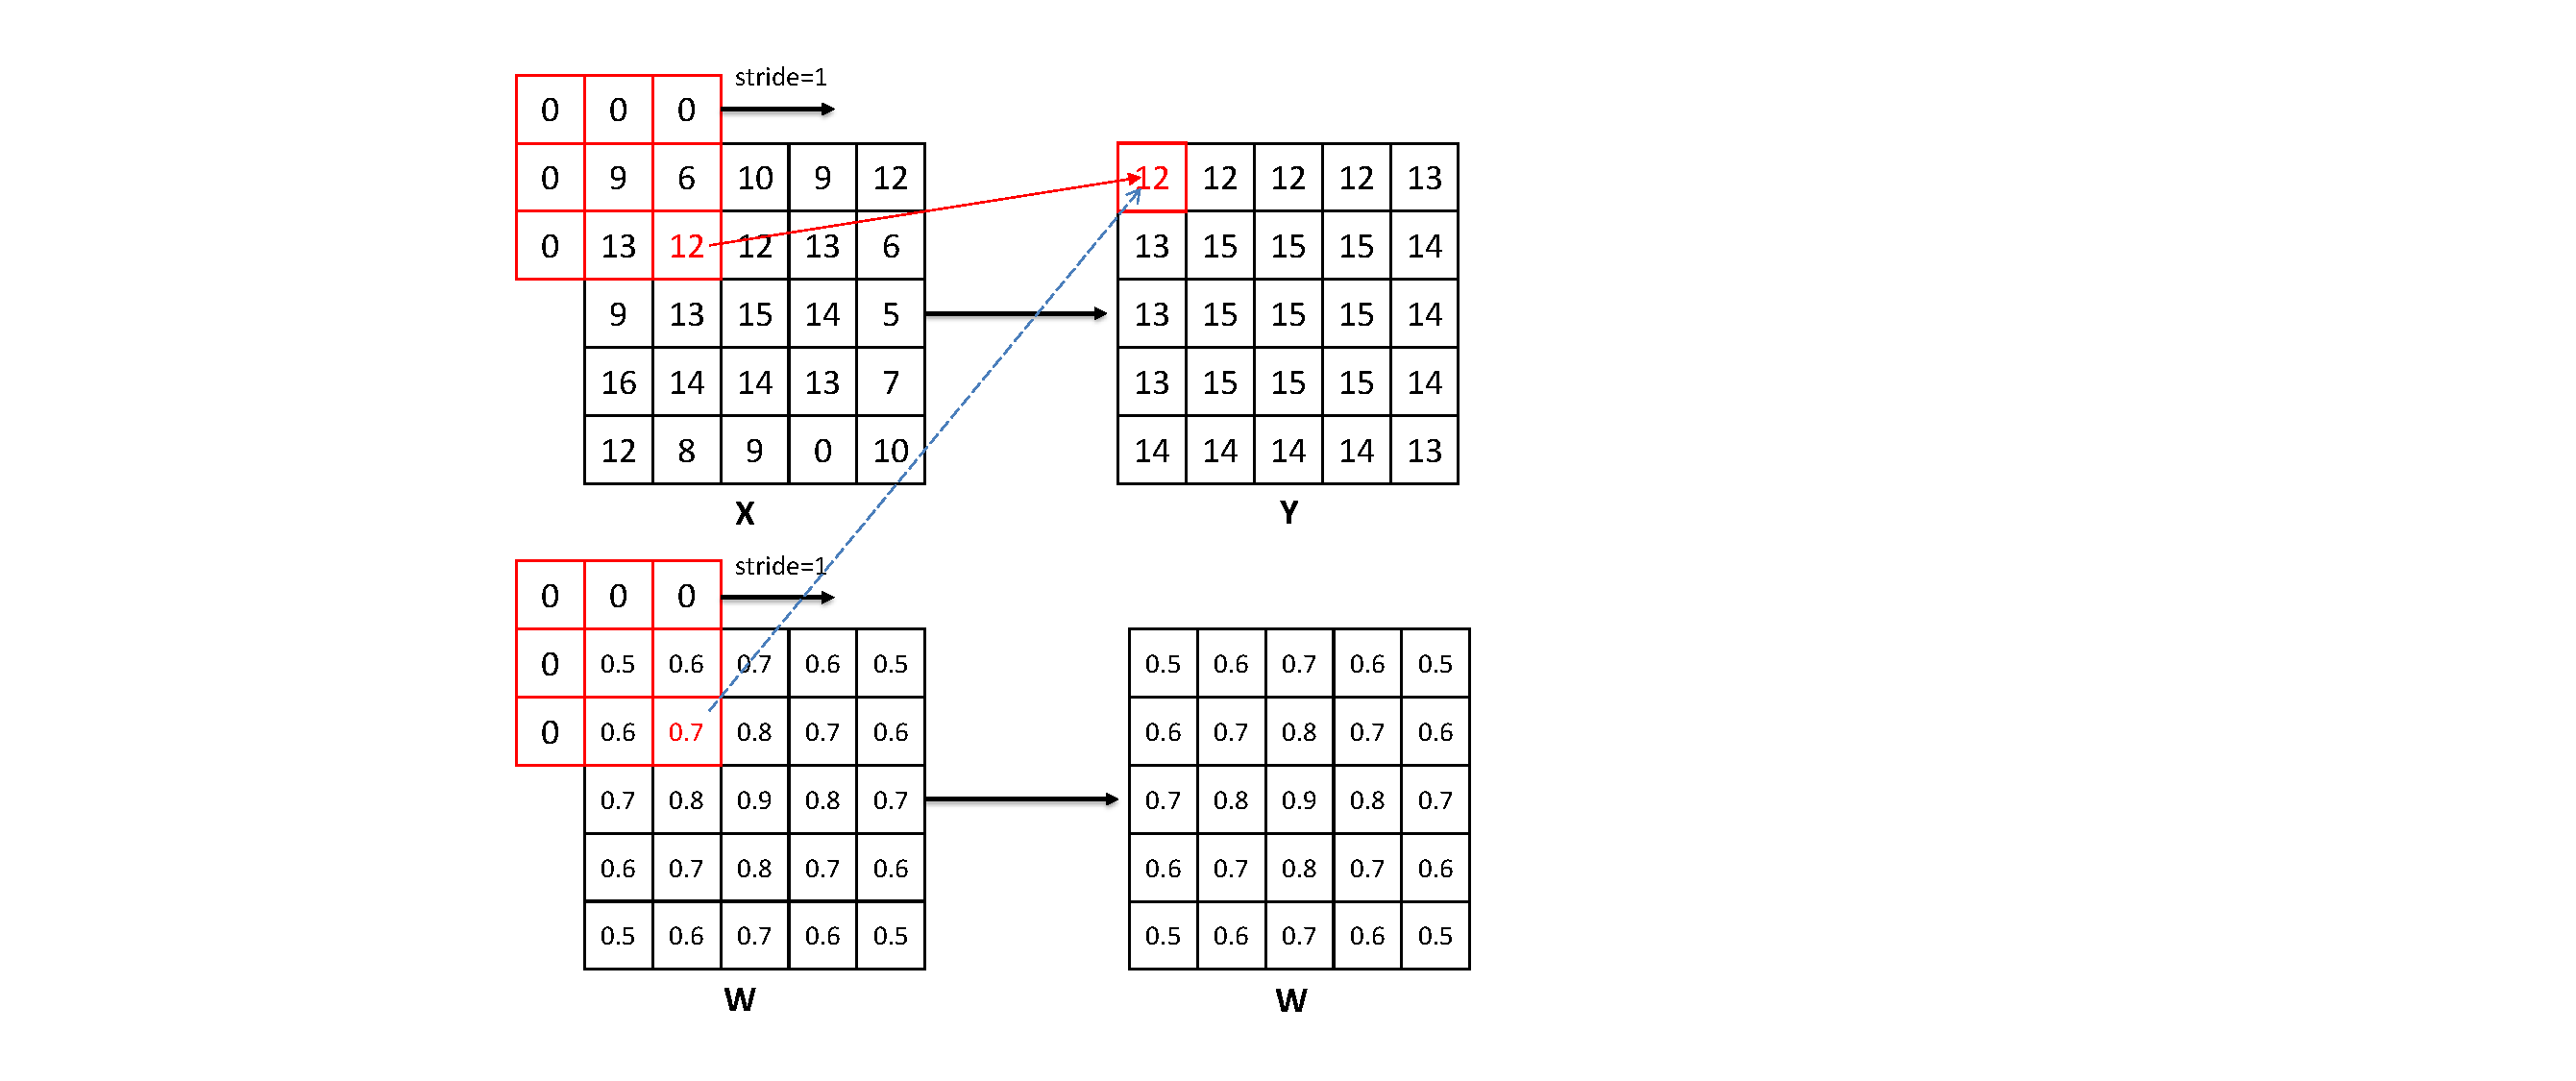
\includegraphics[width=3.4in]{figures/FigJMP.pdf}
   %\includegraphics[width=0.8\linewidth]{egfigure.eps}
    \end{center}
    \caption{An example of joint max pooling.
        Two windows of same size synchronously slide on $\mathbf{X}$ and $\mathbf{W}$.
       The elements in top window will be propagated the element under the indicator of bottom window.}
    \label{FigJMP}
\end{figure}

Based on this observation, we proposed a joint pooling layer \bobo{change a more accurate name?} by separating $\omega$ apart, rather than depend on $x$ or be fixed.
Explicitly, our joint pooling take two inputs, respectively denoted as $X$ and $W$ with same width and height.
During forward propagation, two windows with same size synchronously slide on $X$ and $W$, which are respectively denoted as $\mathcal{N}^{x}$ and $\mathcal{N}^{\omega}$.
Especially, $\mathcal{N}^{x}$ and $\mathcal{N}^{\omega}$ correspond to the same neighbor region $\mathcal{N}$ on different input maps.
The elements in $\mathcal{N}^{\omega}$ determine which elements in $\mathcal{N}^{x}$ will be propagated to next layer.
A simple example is illustrated in Figure~\ref{FigJMP}.

For max pooling, since $\omega_i$ is hard to be directly learned to be binary, a threshold function $\hbar(\cdot)$ is applied to $\omega_{i}$ by:
\begin{eqnarray}\label{jmp}
\begin{aligned}
y_{j} &= \sum_{i\in \mathcal{N}_{j}}x_{i}\hbar(\omega_{i},\mathcal{N}^{\omega}_{j})\\
\hbar(\omega_{i},\mathcal{N}^{\omega}_{j})&=\left\{\begin{array}{cc}
1&if~\omega_{i}\geq max(\mathcal{N}^{\omega}_{j})\\
0&else\\
\end{array}\right.
\end{aligned}
\end{eqnarray}
where $max(\cdot)$ finds the max value of the input.

It should be noted that in Figure~\ref{FigJMP} that elements $x_i$ in $X$ with small $\omega_i$ have been abandoned and substituted by $x_i$ with larger $\omega_i$ in $Y$.
If this processing is iterated more times, all the elements in $Y$ will be substituted by the $x_i$ with maximum $\omega_i$.
Back to our object segmentation task, it is reasonable to believe that objectness score $p_i$ in central region of an object are probably a local maximum point.
Therefore applying JMP to both outputs from multi-task FCN can well replace the predicted shape parameters in border area of an object with a nearest predictions in central area, which usually have local maximum $p_i$.
Explicitly, $p$, $t$ respectively corresponds to $W$, $X$, while $t$ is pooled under indication of $p$.
The pooling stride is fixed to be $1$ to maintain an unchanged resolution of final segmentation.
Pooling size and iteration times of JMP determine how far the $t_i$ with maximum $p_i$ can be spread.


Moreover, another contribution of our JMP is that the residual error can be correctly back propagated to its inputs.
This makes it a trainable layer in any network architecture and our SCNN become a fully trainable system.
Defining $L_{X}$ as the residual error on $X$ , the back propagation for $x_{i}$ can be expressed by:
\begin{eqnarray}\label{bpx}
\begin{aligned}
\frac{\partial L_\mathbf{X}}{\partial x_{i}}=\frac{1}{m}\sum\limits_{j\in\mathcal{N}_{i}}\frac{\partial L_{X}}{\partial y_{j}}\hbar(\omega_{i},{\mathcal{N}}^{\omega}_{j})\\
\end{aligned}
\end{eqnarray}
where $\mathcal{N}^{\omega}_{j}$ is the neighbor region centered on position $j$ in $W$ and $m$ is the size of $\mathcal{N}_{i}$.
Similar to forward propagation in original max pooling, Eq.~\ref{bpx} converge the gradients $\frac{\partial L_\mathbf{X}}{\partial y_{j}}$ into $x_{i}$ which has a local maximum $\omega_{i}$.
In this way, as most residual error $\frac{\partial L_\mathbf{X}}{\partial y_{j}}$ have been focused on area with high objectness scores by Eq.~\ref{bpx}, the predicted shape parameters in central area of objects will be more accurate.

%Specially in Figure \ref{FigSCNN}, the input segmentation map is assumed to not only influence the output but also feeds a subsequent layers, thus also receiving gradient contributions $\frac{\partial L}{\partial s_{i,j}}$ from the next layer during back-propagation.

Defining $L_{W}$ as the residual error on $W$.
It should be noted that our JMP will be iterated several times to spread $x_{i}$ with local maximum $\omega_{i}$ farther.
Therefore, we assume that $\omega_{i}$ not only influences the following $\{y_{j}|j\in\mathcal{N}_{i}\}$, but also receiving gradient contributions $\frac{\partial L_W}{\partial \omega_{i}}$ from subsequent JMP layer or shape supervised label during back-propagation.
The back propagation for $\omega_{i}$ is formulated by
%
\begin{eqnarray}\label{bps}
\begin{aligned}
\frac{\partial L_{W}}{\partial \omega_{i}}&=\frac{\partial L_{W}}{\partial \omega_{i}}+\frac{1}{m}\sum_{j\in\mathcal{N}_{i}}\frac{\partial L_{W}}{\partial y_{j}}\frac{\partial y_{j}}{\partial \omega_{i}}\\
&=\frac{\partial L_{W}}{\partial \omega_{i}}+\frac{1}{m}\sum_{j\in\mathcal{N}_{i}}\frac{\partial L_{W}}{\partial y_{j}}x_{i}\frac{\partial \hbar(\omega_{i},\mathcal{N}^{\omega}_{j})}{\partial \omega_{i}}\\
&=\frac{\partial L_{W}}{\partial \omega_{i}}+\frac{1}{m}\sum_{j\in\mathcal{N}_{i}}\frac{\partial L_{W}}{\partial y_{j}}x_{i}\delta(\omega_{i},\mathcal{N}^{\omega}_{j})\\
\end{aligned}
\end{eqnarray}
where $\delta(\omega_{i},\mathcal{N}^{\omega}_{j})$ is the derived function of $g(\omega_{i},\mathcal{N}^{\omega}_{j})$, which has an infinite response when $\omega_{i}$ is the maximum in $\mathcal{N}^{\omega}_{j}$.
In order to robustly propagate gradients to $\omega_{i}$, $\frac{\partial L_{W}}{\partial y_{j}}x_{i}$ is approximated by $\frac{\partial L_\mathbf{W}}{\partial \omega_{i}}$ multiplying a constant value $\alpha$  and $\delta(\omega_{i},\mathcal{N}^{\omega}_{j})$ is approximated to be $\hbar(\omega_{i},\mathcal{N}^{\omega}_{j})$.
Therefore, $\frac{\partial L_{W}}{\partial \omega_{i}}$ is formulated as a more concise form:
\begin{eqnarray}\label{dG}
\begin{aligned}
\frac{\partial L_{W}}{\partial \omega_{i}}&=\frac{\partial L_{W}}{\partial \omega_{i}}(1+\frac{1}{m}\sum_{j\in\mathcal{N}_{i}}\alpha \hbar(\omega_{i},\mathcal{N}^{\omega}_{j}))\\
\end{aligned}
\end{eqnarray}

Intuitively, Eq. \ref{dG} adds a loss weight on gradients of the local maximum $\omega_{i}$ with control of $\alpha$, which is beneficial to avoiding false and missing detection .

\subsection{Local Optimization for Final Segmentation}
\label{sec:fusion}
Based on the objectness map and auxiliary map of shape parameters obtained from joint max pooling, we now integrate the two types of information to produce more accurate boundaries.
Especially, the shape of objects in objectness map are predicted unrestrictedly by neural network without shape knowledge, while the shape of objects in auxiliary map are strictly constrained.
Therefore, it is important to reasonably fuse these two kinds of information into final segmentation mask.

In this section, a local optimization strategy is applied to allow our method to not only optimize the shape of regular objects, but also accommodate seriously deformable objects.
A key assumption in our local optimization strategy is that the shape of objects predicted in objectness map is approximate to the ground truth.
Hence we coarsely divide an objectness map into three parts: object area, contour area and background area.
The contour area is the ambiguous regions that is not sure to belong to object or background area.
In final segmentation mask, only the pixel in contour area are classified by predicted shape parameters, while the remaining pixels are classified by objectness scores.
For example with an objectness score $p_i$ and a set of parameters $t_i$ at position $i$, the classification result $m_i$ for pixel $i$ is determined by:
%
\begin{eqnarray}\label{fusion}
\begin{aligned}
m_i=\left\{\begin{array}{cc}
1&if~p_i>\tau_2\\
0&if~p_i<\tau_1\\
f(t_i)&else\\
\end{array}\right.
\end{aligned}
\end{eqnarray}
where $\tau_2$ and $\tau_1$ are two thresholds (set empirically) to control the degree of modification by prior shape constraint.
$f(t_i)$ is a function judging whether the pixel $i$ is within an object formulated by $t_i$.
As in our task an ellipse is defined by $ t_i = [\theta, \mu_c, \nu_c, a, b]$, the function is expressed by:
\begin{eqnarray}\label{fusion}
\begin{aligned}
f(t_i)&=\left\{\begin{array}{cc}
1&if~\frac{d\mu^2}{a^2}+\frac{d\nu^2}{b^2}<1\\
0&else\\
\end{array}\right.\\
dx &= cos(\theta)(\mu-\mu_c)+sin(\theta)(\nu-\nu_c)\\
dy &= -sin(\theta)(\mu-\mu_c)+cos(\theta)(\nu-\nu_c)\\
\end{aligned}
\end{eqnarray}
where $\mu$, $\nu$ are the spatial coordinates of pixel $i$. 

Our fusion strategy can appropriately utilize prior shape knowledge to not only separate touching objects into individual ones, but also optimize most regular object without losing generalization to deformable objects.
And our SCNN can be easily extended to other shape constraint, such as rectangle shape, circles by changing the form of shape parameters.

\section{Experiments}
\label{sec:results}
To demonstrate our superiority over existing methods on segmentation, we first present results on two diverse biomedical image segmentation problems, including synaptic vesicle segmentation and gland segmentation.
To demonstrate the easy extension and generic applicability of our framework, we modified our SCNN to scene text segmentation task.

\subsection{Synaptic vesicle segmentation}
\noindent\textbf{Dataset}
Synaptic vesicle is a good example to evaluate our method, as most of vesicle shape are ellipse.
The images were acquired by . \cxj{by what?}
However synaptic vesicle images are much noisy due to deficient imaging technique.
The plausible vesicles in image are densely arranged and easily confused with other membrane in presynaptic cell, therefore it is hard to obtain clear contour for such dense and small objects.
%The ground truths of dataset are held out by biologists for objective evaluation.
The original dataset is composed of $120$ images with annotations provided by biologists.
The height and width of each image are respectively $1019$ and $1053$, averagely containing $200$ vesicle objects.
Since the average length of a vesicle is about $30$ pixel, we crop a $321\times 321$ region following \cite{Chen2014a} from the original image as the input to network so that each cropped image contain about $25$ objects.
We uniformly crop $25$ patches in each original image with overlap, then the final dataset consists of $3000$ images of $321\times 321$ resolution.

Similar with many existing approaches, we utilize a data augmentation process to reduce overfitting and increase the robustness of our network.
In data augmentation, translation, rotation and image flipping are used to finally produce $8787$ images for training and evaluation.
%\cxj{The final dataset size?}
For better evaluation, a six-fold cross validation is applied in our experiments.
%The first five out of six images are prepared to train our model and the rest of them are used to test its performance.
%\cxj{Six-fold cross validation? or other strategy? }
%
%The validation processing has been repeated several times and the average performance will be reports.


\noindent\textbf{Implementation details.}
We train our network on the open-source deep learning library Caffe~\cite{Jia2014}.
%All the experiments are implemented on a workstation with TitanX GPU cards.
The model of SCNN is well trained by two-step process.
In first stage, we independently train the segmentation branch and shared layers as a general segmentation task.
The parameters of shared layers are initialized from VGG-16 ImageNet pretrained model.
During training phase, the base learning rate was set as $10^{-3}$ and a `step' policy is adopted by decreasing the learning rate by a fact of $10$ every $2000$ iterations.
And mini-batch size was set to $30$ for one iteration with the max iteration number $20000$.
In the second stage, the multi-task FCN as well as two successive joint max pooling layers is jointly fine-tuned based on the model from first stage.
The learning rate of new added layers was set as $10^{-5}$, while the other learning rate was set to $10^{-8}$.
The iteration number of training in second stage is set as $8000$.
Especially, joint max pooling requires multiple iterations $L$ to optimize as many shape predictions in boundary area as possible.
And the optimal $L$ together with pooling size $k_s$ will be jointly explored in subsequent experiment.
The balancing weight $\alpha$ in Eq.~\ref{EqLoss} was determined by fixing $\alpha L=20$, of which the value $20$ is calculated according to the ratio of positive and negative labels of the whole dataset.
For fusing step, the important thresholds $\tau_1$ and $\tau_2$ are also explored in latter experiment, which determine the degree of prior shape constraint in final segmentation mask.

\noindent\textbf{Evaluation setup.}
%
The evaluation criteria in our experiments includes an score $F_1$ to evaluate performance of object detection and a pixel intersection-overunion (IOU) averaged across different classes to evaluate the segmentation accuracy .
%The $F_1$ score considers the performance of object detection, while IOU consider the segmentation performance, respectively.

For detection, the $F_1$ score is defined as:
%
\begin{eqnarray}\label{EqF1}
\begin{aligned}
F1 = \frac{2PR}{P+R}
\end{aligned}
\end{eqnarray}
where $P$ is the detection precision and $R$ is the detection recall.
Especially, a true positive detection is the segmented object that intersects with at least $50\%$ with the ground truth, otherwise it is regarded as a false positive.
If a ground truth object has no corresponding segmented object that intersects more than $50\%$, it is regarded as a false negative.

The IOU metric for segmentation accuracy is defined as:
%
\begin{eqnarray}\label{EqIou}
\begin{aligned}
IOU = \frac{1}{N_s}\sum_{i=1}^{N_s}\frac{|G_i\bigcap S_i|}{|G_i\bigcup S_i|}
\end{aligned}
\end{eqnarray}
%
where $N_s$ denotes the number of pixel label.
$G_i$ denotes the pixel set with $i$-th label in ground truth .
$S_i$ denotes the pixel set with $i$-th class in segmented result.
In our object segmentation task, there are two kind of labels: object or background, therefore $N_s$ is set to $2$.
\begin{figure*}
    \begin{center}
        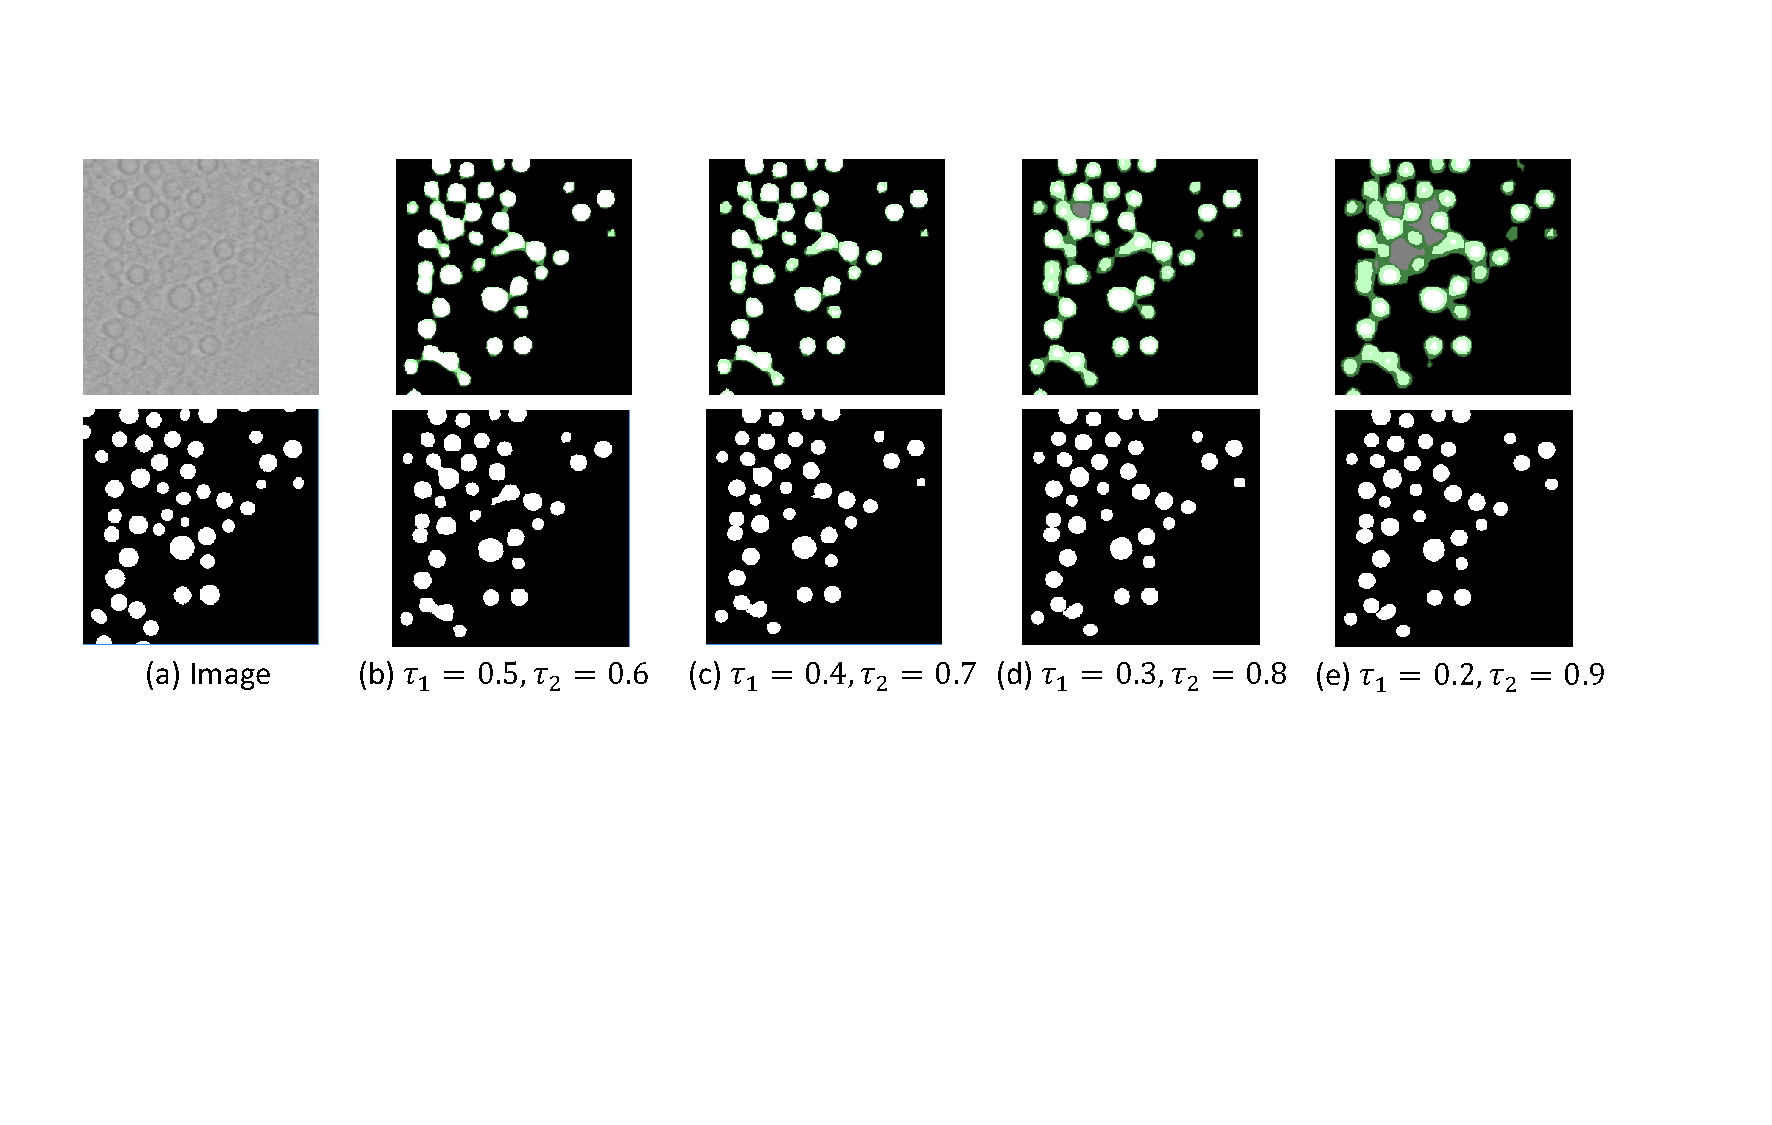
\includegraphics[width=7in]{figures/FigCon.pdf}
    \end{center}
    \caption{Effect of varying fusion thresholds $\tau_1$ and $\tau_2$ with $\varepsilon=9$. First row contains the input image and raw segmentations from bojectness score, where the pixels of objectness score between $[\tau_1,\tau_2]$ has been highlighted. Second row contains the ground truth and optimized segmentations of varying $[\tau_1,\tau_2]$. It shows that a large interval of $[\tau_1,\tau_2]$ means the stronger shape constraints to the segmented objects.}
    \label{FigCon}
\end{figure*}


\begin{figure*}
    \begin{center}
        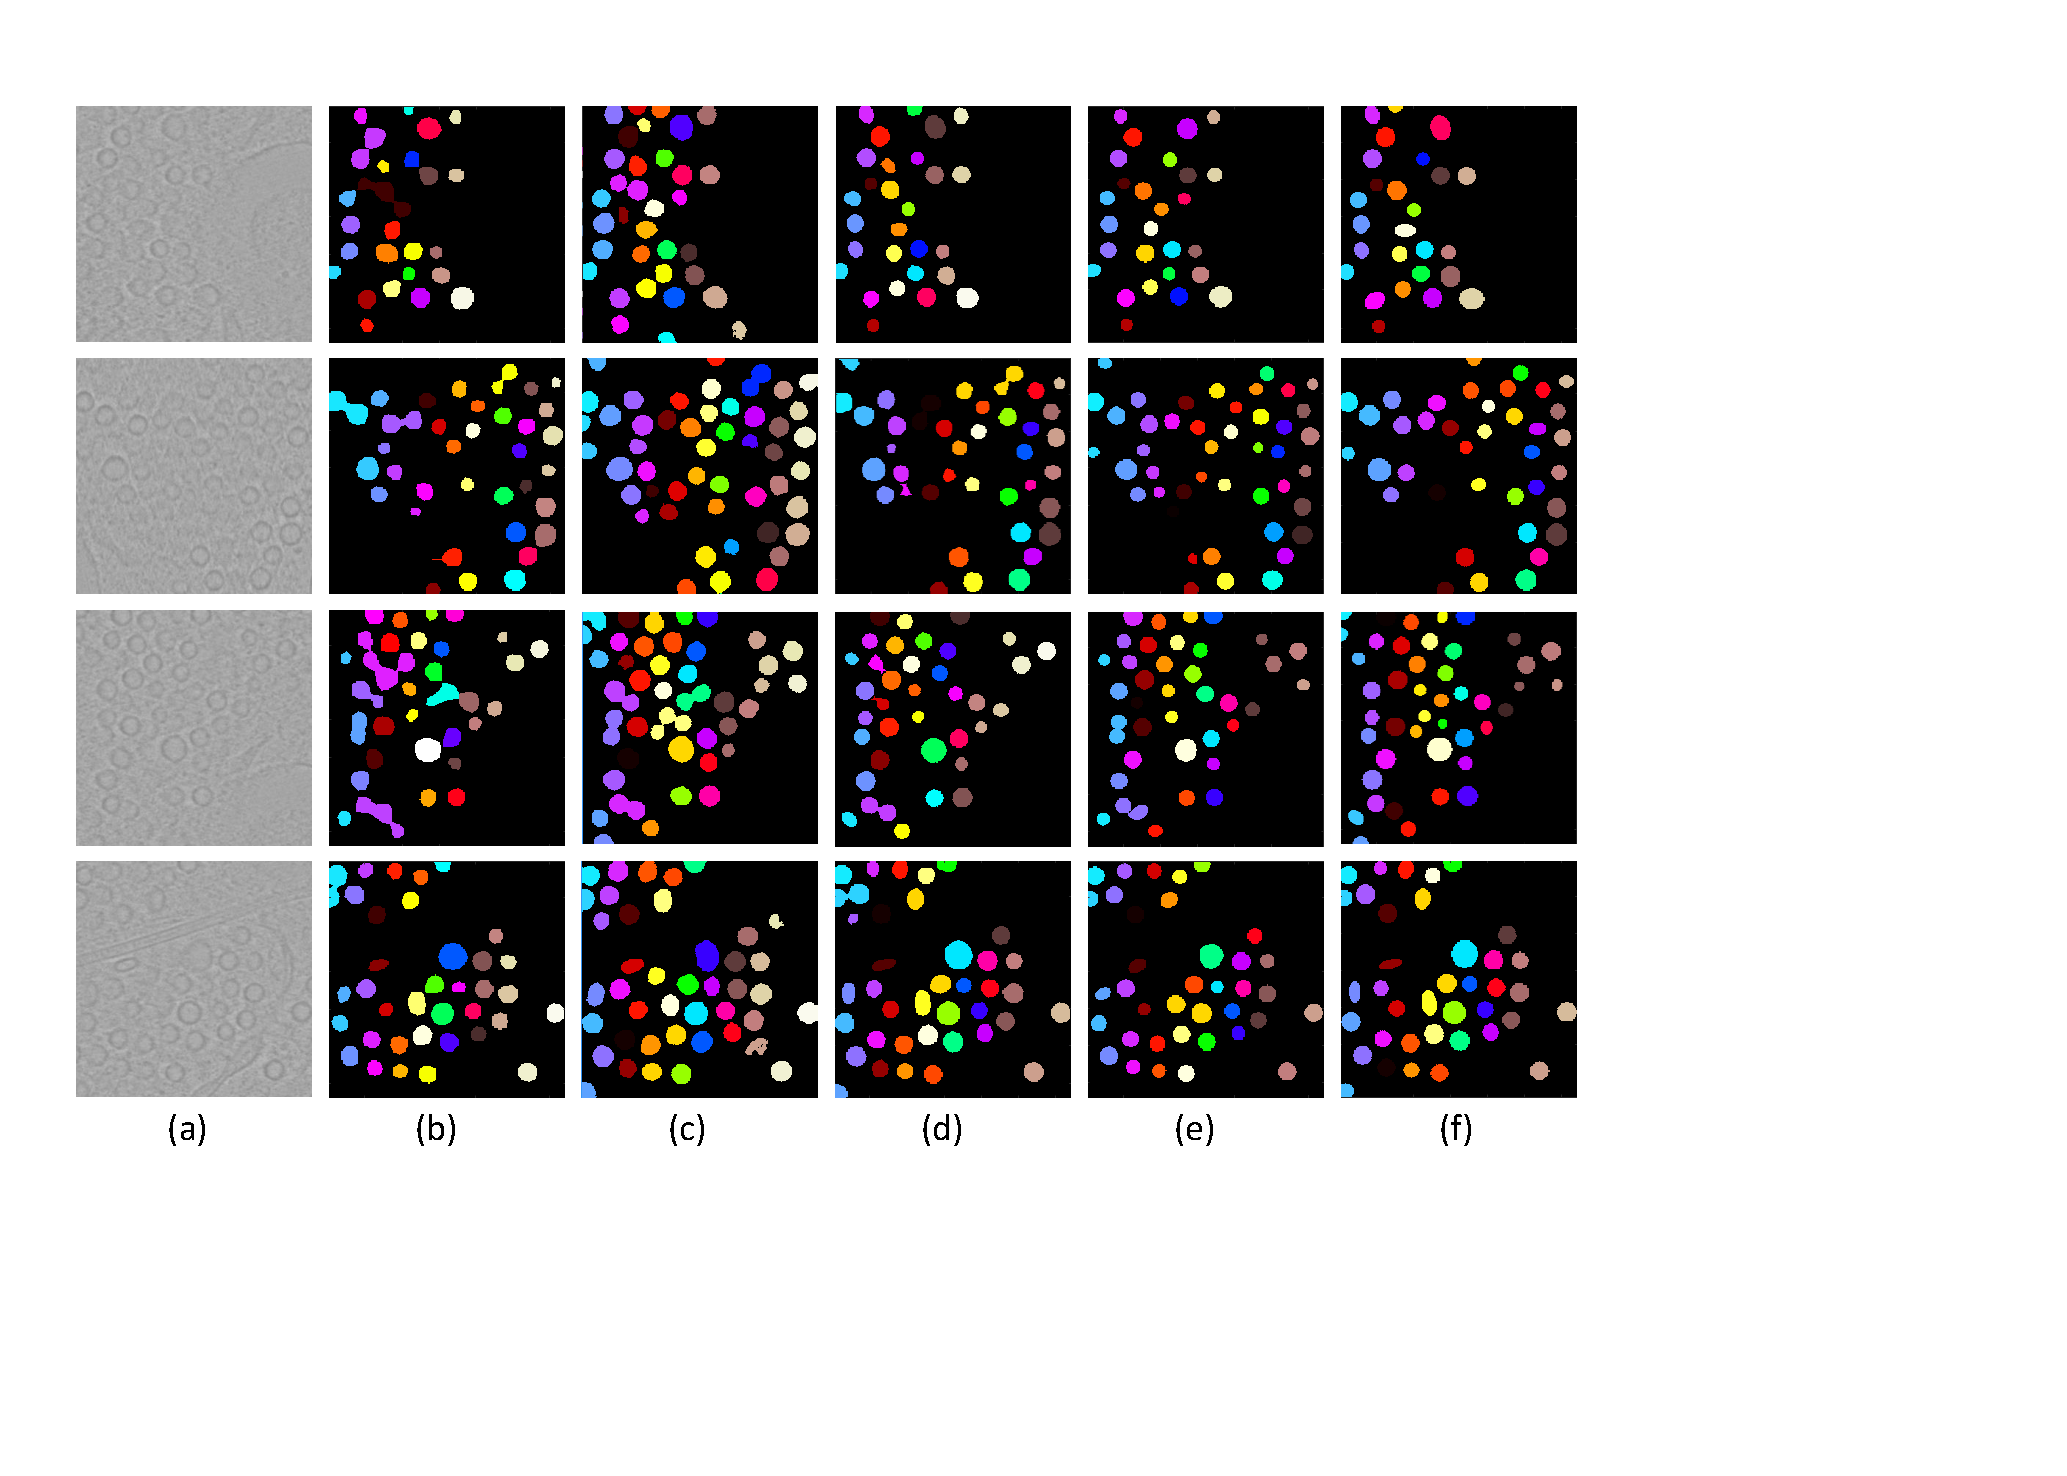
\includegraphics[width=7in]{figures/FigVesicle.pdf}
    \end{center}
    \caption{Some segmentation results of synaptic vesicle: (a) the input image; (b)-(f) the segmentation respectively from deeplab, u-net, DCAN, $SCNN^{-1}$ and SCNN; (g) the ground truth.}
    \label{FigVesicle}
\end{figure*}

\noindent\textbf{Exploring the effect of $\{L, k_s, \tau_1, \tau_2\}$ to final segmentation.}
In this experiment, the effect of different $L$, $k_s$, $\tau_1$, $\tau_2$ for segmentation performance is jointly investigated and the optimal solution will be searched.
In order to reduce the hyper-parameters, we use $\varepsilon=\frac{(L-1)k_s}{2}$ to simultaneously represent $L$ and $k_s$ , because the influence of both $L$ and $k_s$ to the whole network is the reception field of joint max pooling layers.
Therefore, we first fix $\tau_2=0.7$ and vary $\tau_1$ to observe its effect of different $\varepsilon$ as shown in Figure~\ref{FigVar} (a).
Then, $\tau_1$ is fixed in turn and $\tau_2$, $\varepsilon$ are varied in Figure~\ref{FigVar}  (b).
Observed from Figure~\ref{FigVar} , it is properly to employ $\varepsilon=9$ for vesicle segmentation to obtain most of the gains for different $\tau1$ and $\tau2$.
In practice, we set $k_s=9$ and $L=3$ to satisfy the condition of $\varepsilon=9$, which reaches a balance between speed and effect.
For $\tau_1$ in Figure~ (a), we fine that $\tau_1=0.2$ is the best lower threshold when $\varepsilon=9$.
And fixing $\tau_1=0.2$, $0.9$ is found to be the optimal value of $\tau_2$ according to Figure~\ref{FigVar} (b).
Finally, we use a large interval of $[0.2, 0.9]$ as the thresholds in Eq.~\ref{fusion} to impose a strong shape restriction, because the shape of most synaptical vesicles are regular ellipse.
Especially, $\varepsilon=0$ means no joint max pooling applying to network.
Besides finding the optimal values of $\tau_1$ and $\tau_2$, it can be found that the segmentation accuracy is coarsely positive correlation to $\varepsilon$ in  Figure~\ref{FigVar} .
This demonstrate the effectiveness of our JMP in improving the accuracy of predicted shape parameters in boundary area with increasing $\varepsilon$.
And an interesting observation is that the effect of varying $\tau_2$ to final segmentation is not as obvious as varying $\tau_1$.
This is because that most misclassified pixels comes from the touching area, whose objectness scores $P_i$ are lower and approximate to $0.5$ shown in Figure~\ref{FigVesicle}.
Furthermore, we presents some examples of different $[\tau_1,\tau_2]$ in Figure~\ref{FigCon} to illustrate how these thresholds control the degree of prior shape constraint to segmented objects.

\begin{figure}
    \begin{center}
        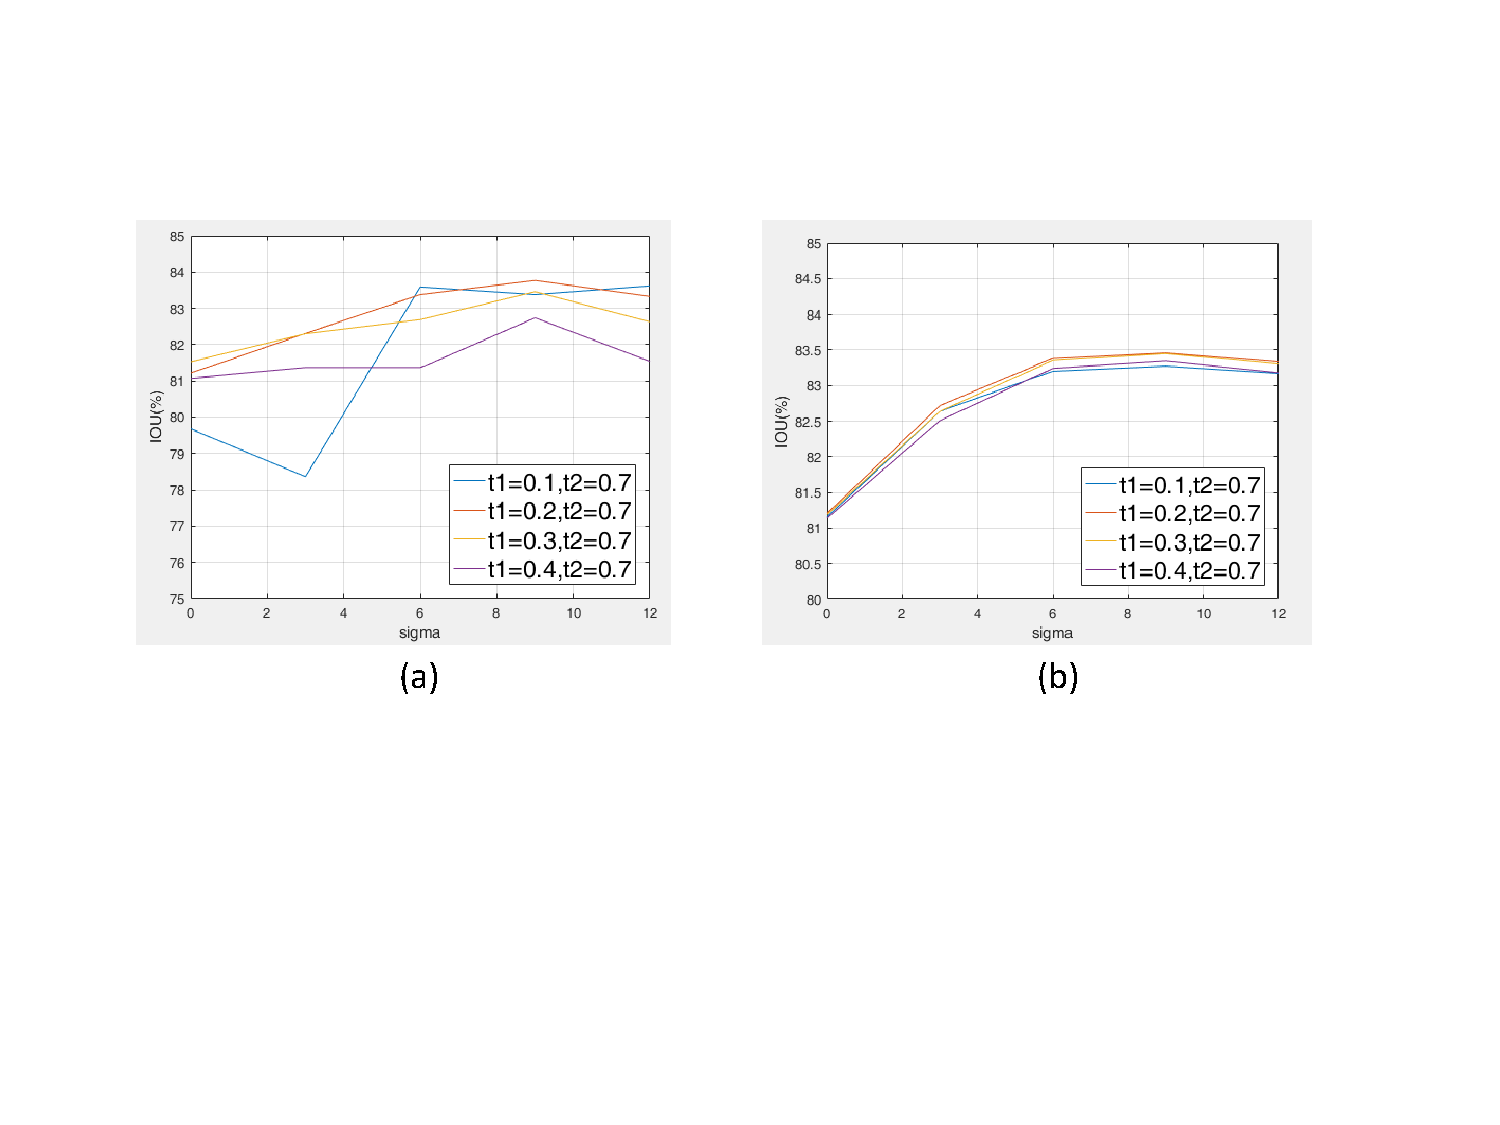
\includegraphics[width=3.5in]{figures/FigVar.pdf}
   %\includegraphics[width=0.8\linewidth]{egfigure.eps}
    \end{center}
    \caption{Effect of varying $\varepsilon$ for vesicle segmentation: (a)Fix $\tau_2$ and vary both $\tau_1$ and $\varepsilon$. (b) Fix $\tau_1$ and vary both $\tau_2$ and $\varepsilon$.}
    \label{FigVar}
\end{figure}

\noindent\textbf{Qualitative evaluation on synaptic vesicle segmentation}
Figure \ref{FigVesicle} shows some segmentation results of testing data.
In order to verify the effectiveness of parameterized shape information, we compared our method with DeepLab \cite{Chen2014a}, u-net~\cite{Ronneberger2015} without any complementary information and DCAN~\cite{Chen2016a} with contour map as auxiliary.
Furthermore, we also present the results of $SCNN^{-}$ that remove the joint max pooling layers from SCNN to prove its effectiveness.
The fusing thresholds follow the optimal setting in previous experiment.

From Figure \ref{FigVesicle}, we can see that without other complementary information, there exists many touching objects that cannot be separated by DeepLab (Figure~\ref{FigVesicle} (b)).
This is because that the contours of many synaptic vesicles are very fuzzy and incomplete due to deficient imaging technique as shown in Figure~\ref{FigVesicle} (a).
And the dense synaptic vesicles around presynaptic membrane increase the difficulty to separate them into individual ones.
Also without auxiliary, u-net (Figure~\ref{FigVesicle} (c)) is superior than DeepLab in terms of touching problem due to the U-shape network that supplements many context information to higher resolutions layers.
However, the raw context information added to higher layers brings more false detection into the segmentation, because of the coarse raw image quality.
Although DCAN is capable to separate touching synaptic vesicles apart in Figure~\ref{FigVesicle} (e), it also produced additional false detections by cutting the touching vesicles with respective contours.
When the connection region between two touching vesicles are wide and large, cutting the touching regions by respective contours will generate an additional positive region besides two separated vesicle objects.
Differen from the above methods, our SCNN uses the shape parameters of objects as complementary information to separate the touching object clearly without residual regions.
As the results in Figure~\ref{FigVesicle} (f), all the touching objects have been well separated and their shape are more smooth and regular.
And the comparing result of Figure~\ref{FigVesicle} (e) prove again the effectiveness of joint max pooling by improving the accuracy of shape parameters.

\noindent\textbf{Quantitative evaluation.}
To quantitatively evaluate our method, we compare the object detection rate $F_1$ and the segmentation accuracy IOU of our SCNN with the state of the art segmentation methods based on Deeplab~\cite{Chen2014a}, u-net~\cite{Ronneberger2015} and DCAN~\cite{Chen2016b}, which are commonly used in biomedical image process.
Their results on our synaptic vesicle dataset are shown in Table~\ref{tab:vesicle}.
And we further implement $SCNN^{-}$ that is the clipped version of SCNN without joint max pooling.
Their results are also presented in Table~\ref{tab:vesicle} to prove effectiveness of our joint max pooling.

From F1 score obtained in Table~\ref{tab:vesicle}, the performance of SCNN surpassed the other methods.
The common low F1 scores are caused by difficulty in detecting dense synaptical vesicles in such noise background.
Especially, we observed that the performance of u-net obtained about $3\%$ improvement over DeepLab, both of which did not use any auxiliary supervised information.
This arises from the fact that U-shape applied in u-net is effective to alleviate touching problem, which confirmed that missing of context information is a significant factor of touching problem in biomedical segmentation.
Furthermore, we noticed that there is not much improvement of F1 score obtained by DCAN compared to u-net and DeepLab.
This is because that many false detection region between two objects, separated by predicted contours, increase the false positive scores in Eq.~\ref{EqF1}, shown in Figure~\ref{FigVesicle} (d).
And $SCNN_{-}$ gives a lower F1 score compared to SCNN, because of some touching cases caused by inaccurate auxiliary information predicted in boundary area.

From IOU metrics in Table~\ref{tab:vesicle}, our SCNN gives the best performance again among various methods.
It should be noted that although the other methods also obtain a good IOU score, their contours are more coarse and irregular as shown in Figure~\ref{FigVesicle}, which increase the difficulty of subsequent processing such as reconstruction of 3D structure.
And the segmented vesicle by our SCNN are more clear and regular.
Moreover, the results demonstrate that our joint max pooling operation can effectively improve the accuracy of predicted shape parameters, which leads to a better performance on objects shape.
Both qualitative and quantitative evaluations present the superiority of our SCNN in segmenting densely arranged objects with regular and small objects by incorporating the prior shape knowledge into network.

\begin{table}
\begin{center}
\begin{tabular}{lcc}
\hline
Method & F1($\%$) & IOU($\%$) \\
\hline
DeepLab & 66.75 & 80.95 \\
U-net & 69.99 & 77.56 \\
DCAN & 70.94 & 80.61 \\
$SCNN^{-}$ & 74.52 & 81.04 \\
SCNN & $\mathbf{75.68}$ & $\mathbf{83.34}$\\
\hline
\end{tabular}
\end{center}
\caption{The detection and segmentation results of different methods in our synaptic vesicle dataset.}
\label{tab:vesicle}
\end{table}

\subsection{Gland segmentation}
\textbf{Dataset}
In this section we present SCNN for segmenting benign and malignant gland.
We consider the public dataset of \emph{Gland Segmentation Challenge Contest} in MICCAI2015~\cite{Sirinukunwattana2015a}.
%
The training dataset is composed of 85 images, consisting of 37 benign and 48 malignant, with ground truth annotations provided by expert pathologists.
Especially, there is a huge variation of glandular morphology in malignant case, which can prove the generalization of our SCNN to irregular objects.
The same data augmentation in vesicle segmentation is implemented for a better performance.

\textbf{Implementation details}
Because there exists many irregular objects in gland images that we desire to remain more contour information obtained by object prediction, the contour modification by parameterized contour information should be relatively weaker than segmenting vesicles.
By experimental verification, we find that $\tau_2=0.7$ and $\tau_1=0.4 $ produce a better results.
\cxj{So show comparison of results using different parameters.}
%
And we still use the standard elliptic parameter as the prior shape constraint for gland, as most benign glands and few malignant glands' shape are approximate ellipses.
The other implementation settings and evaluation metrics follow the vesicle segmentation.

\textbf{Qualitative evaluation on gland segmentation}
Follow previous qualitative evaluation, we presented the results of u-net and the state of art method DCAN in gland segmentation with our SCNN in Figure~\ref{fig:com-gland}.
The first two columns are the examples of benign gland images, and the rest two columns are the examples of malignant images.
From the results, we can observed that both SCAN and SCNN can well solve the touching problem in benign and malignant cases.
However for benign case, the contours of glands obtained by SCNN are more smooth than that of DCAN.
And for malignant case, since SCNN only modify the segmentation predictions on the object border, there is no obvious deterioration compared to DCAN.

\begin{figure}
	\centering
	\vspace{0.4in}
	\caption{\cxj{Add comparison of gland segmentation with U-net and DCAN.}}
	\label{fig:com-gland}
\end{figure}

\textbf{Quantitative evaluation}
Table \ref{} shows the F1 score and IOU metric over the $Gland$ $Segmentation$ $Challenge$ $Contest$ by several commonly used biomedical segmentation methods.

\begin{table}
	\centering
	\caption{Performance comparison on gland segmentation.}
	\begin{tabular}{c|cc}
		\hline
		Method & F1 & IOU \\
		\hline
		DeepLab & 0 & 0 \\
		U-Net & 0 & 0 \\
		DCAN & 0 & 0 \\
		SCNN-v1 & 0 & 0 \\
		SCNN-v2 & 0 & 0 \\
		\hline
	\end{tabular}
\end{table}


\subsection{Scene text detection}
We further extended SCNN to scene text detection task, which


\section{Conclusion}
In this paper, a novel and general method is proposed for incorporating the prior shape knowledge into neural network to segment the plausible objects in biomedial images.
Based on the popular multi-task FCN in segmentation, we replace the auxiliary contour probability with the shape of objects, formulated by a set of meaningful parameters.
In order to improve the accuracy of predicted shape parameters, a novel joint max pooling layer is proposed to replace the predictions in boundary area with those in center of an object.
Finally with our local fusion strategy, the degree of shape constraint can be flexibly adjusted in terms of different tasks.
We experimented our method on two biomedical task for segmenting synaptical vesicles from electron microscope images and the glandular structures from colorectal cancer tissues.
To further prove the generality of our model to diverse shape constraint, we extend our method to the scene text detection task by segmenting the scene text region with regular shape.
All the experiments had demonstrated the effectiveness of our methods on object segmentation with prior shape knowledge.

{\small
\bibliographystyle{ieee}
\bibliography{egbib}
}

\end{document}
